\documentclass{standalone}
\usepackage{tikz}
\usetikzlibrary{patterns, positioning}


\begin{document}
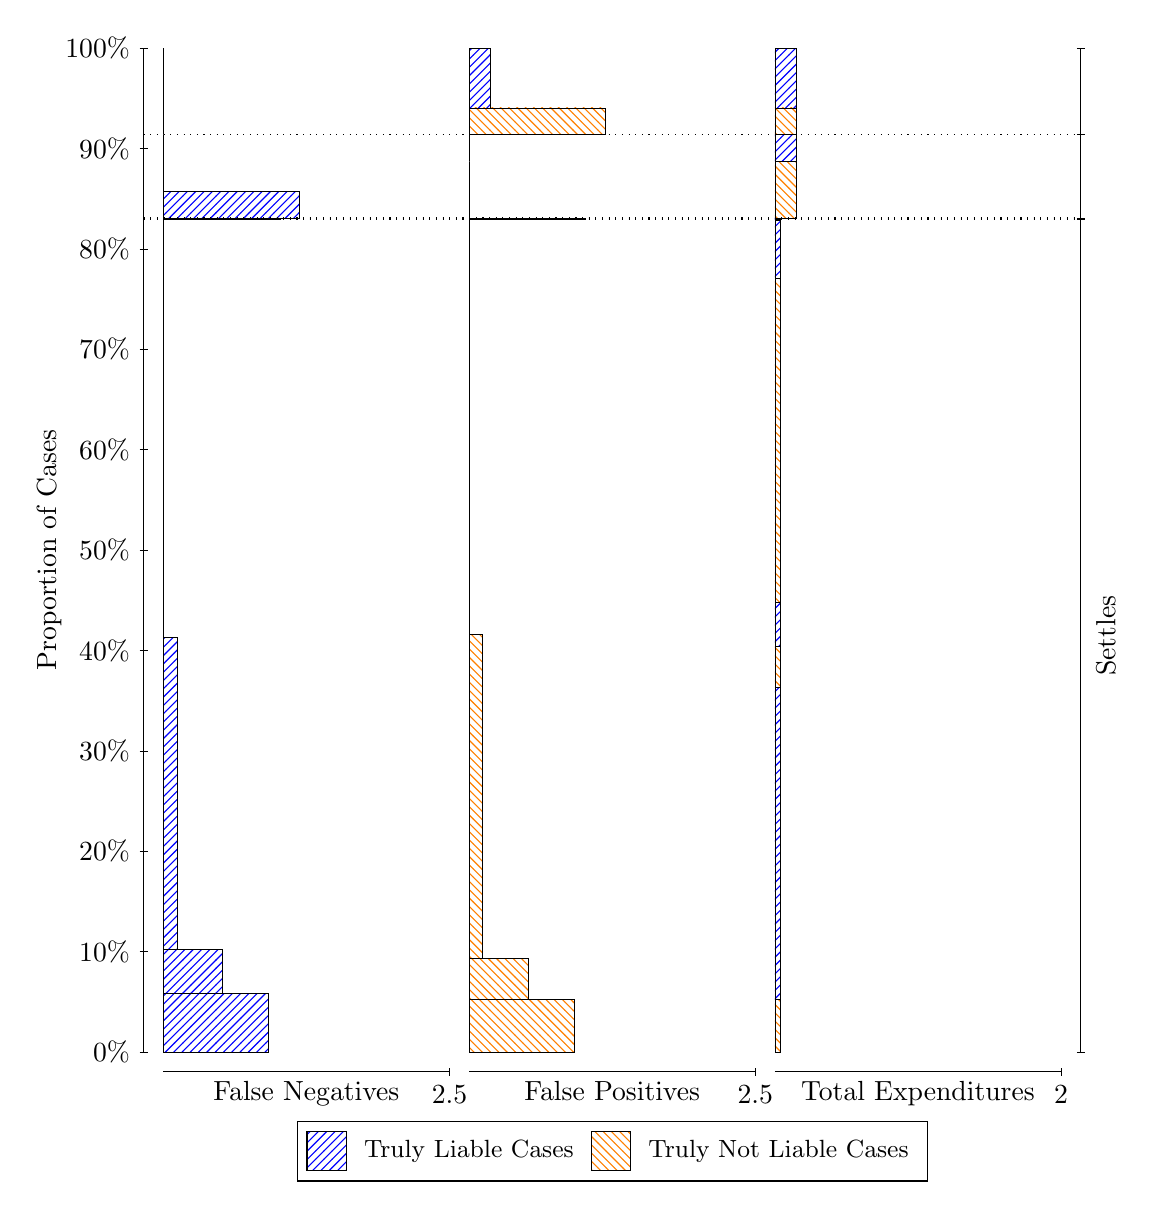
\begin{tikzpicture}
\draw[black, very thin] (1.5,1.75) -- (1.5,14.5);
\node[rotate=90, text=black, anchor=center] at (0.3, 8.125) {Proportion of Cases};
\draw[black, very thin] (1.45,1.75) -- (1.55,1.75);
\node[text=black, anchor=east] at (1.45, 1.75) {0\%};
\draw[black, very thin] (1.45,3.025) -- (1.55,3.025);
\node[text=black, anchor=east] at (1.45, 3.025) {10\%};
\draw[black, very thin] (1.45,4.3) -- (1.55,4.3);
\node[text=black, anchor=east] at (1.45, 4.3) {20\%};
\draw[black, very thin] (1.45,5.575) -- (1.55,5.575);
\node[text=black, anchor=east] at (1.45, 5.575) {30\%};
\draw[black, very thin] (1.45,6.85) -- (1.55,6.85);
\node[text=black, anchor=east] at (1.45, 6.85) {40\%};
\draw[black, very thin] (1.45,8.125) -- (1.55,8.125);
\node[text=black, anchor=east] at (1.45, 8.125) {50\%};
\draw[black, very thin] (1.45,9.4) -- (1.55,9.4);
\node[text=black, anchor=east] at (1.45, 9.4) {60\%};
\draw[black, very thin] (1.45,10.675) -- (1.55,10.675);
\node[text=black, anchor=east] at (1.45, 10.675) {70\%};
\draw[black, very thin] (1.45,11.95) -- (1.55,11.95);
\node[text=black, anchor=east] at (1.45, 11.95) {80\%};
\draw[black, very thin] (1.45,13.225) -- (1.55,13.225);
\node[text=black, anchor=east] at (1.45, 13.225) {90\%};
\draw[black, very thin] (1.45,14.5) -- (1.55,14.5);
\node[text=black, anchor=east] at (1.45, 14.5) {100\%};

\draw[black, very thin] (13.4,1.75) -- (13.4,14.5);
\draw[black, very thin] (13.35,1.75) -- (13.45,1.75);
\node[anchor=west] at (13.35, 1.75) {};
\draw[black, very thin] (13.35,12.32) -- (13.45,12.32);
\node[anchor=west] at (13.35, 12.32) {};
\draw[black, very thin] (13.35,12.331) -- (13.45,12.331);
\node[anchor=west] at (13.35, 12.331) {};
\draw[black, very thin] (13.35,12.342) -- (13.45,12.342);
\node[anchor=west] at (13.35, 12.342) {};
\draw[black, very thin] (13.35,13.401) -- (13.45,13.401);
\node[anchor=west] at (13.35, 13.401) {};
\draw[black, very thin] (13.35,14.5) -- (13.45,14.5);
\node[anchor=west] at (13.35, 14.5) {};

\draw[black, very thin, pattern color=blue, pattern=north east lines] (1.75,1.75) rectangle (3.0852,2.493);
\draw[black, very thin, pattern color=blue, pattern=north east lines] (1.75,2.493) rectangle (2.9399,2.4932);
\draw[black, very thin, pattern color=blue, pattern=north east lines] (1.75,2.4932) rectangle (2.7946,2.4935);
\draw[black, very thin, pattern color=blue, pattern=north east lines] (1.75,2.4935) rectangle (2.6492,2.4938);
\draw[black, very thin, pattern color=blue, pattern=north east lines] (1.75,2.4938) rectangle (2.6492,2.4938);
\draw[black, very thin, pattern color=blue, pattern=north east lines] (1.75,2.4938) rectangle (2.5039,3.0543);
\draw[black, very thin, pattern color=blue, pattern=north east lines] (1.75,3.0543) rectangle (2.3586,3.0551);
\draw[black, very thin, pattern color=blue, pattern=north east lines] (1.75,3.0551) rectangle (2.2133,3.0559);
\draw[black, very thin, pattern color=blue, pattern=north east lines] (1.75,3.0559) rectangle (2.0679,3.0567);
\draw[black, very thin, pattern color=blue, pattern=north east lines] (1.75,3.0567) rectangle (1.9226,7.0149);
\draw[black, very thin, pattern color=orange, pattern=north west lines] (1.75,7.0149) rectangle (1.75,12.32);
\draw[black, very thin, pattern color=blue, pattern=north east lines] (1.75,12.32) rectangle (3.2306,12.324);
\draw[black, very thin, pattern color=orange, pattern=north west lines] (1.75,12.324) rectangle (1.75,12.331);
\draw[black, very thin, pattern color=blue, pattern=north east lines] (1.75,12.331) rectangle (1.7773,12.338);
\draw[black, very thin, pattern color=orange, pattern=north west lines] (1.75,12.338) rectangle (1.75,12.342);
\draw[black, very thin, pattern color=blue, pattern=north east lines] (1.75,12.342) rectangle (3.4758,12.683);
\draw[black, very thin, pattern color=orange, pattern=north west lines] (1.75,12.683) rectangle (1.75,13.401);
\draw[black, very thin, pattern color=orange, pattern=north west lines] (1.75,13.401) rectangle (1.75,13.741);
\draw[black, very thin, pattern color=blue, pattern=north east lines] (1.75,13.741) rectangle (1.75,14.5);
\draw[black, very thin, pattern color=orange, pattern=north west lines] (5.6333,1.75) rectangle (6.9686,2.4186);
\draw[black, very thin, pattern color=orange, pattern=north west lines] (5.6333,2.4186) rectangle (6.8233,2.4189);
\draw[black, very thin, pattern color=orange, pattern=north west lines] (5.6333,2.4189) rectangle (6.6779,2.4193);
\draw[black, very thin, pattern color=orange, pattern=north west lines] (5.6333,2.4193) rectangle (6.5326,2.4196);
\draw[black, very thin, pattern color=orange, pattern=north west lines] (5.6333,2.4196) rectangle (6.3873,2.9398);
\draw[black, very thin, pattern color=orange, pattern=north west lines] (5.6333,2.9398) rectangle (6.2419,2.9398);
\draw[black, very thin, pattern color=orange, pattern=north west lines] (5.6333,2.9398) rectangle (6.2419,2.9404);
\draw[black, very thin, pattern color=orange, pattern=north west lines] (5.6333,2.9404) rectangle (6.0966,2.941);
\draw[black, very thin, pattern color=orange, pattern=north west lines] (5.6333,2.941) rectangle (5.9513,2.9415);
\draw[black, very thin, pattern color=orange, pattern=north west lines] (5.6333,2.9415) rectangle (5.8059,7.0554);
\draw[black, very thin, pattern color=blue, pattern=north east lines] (5.6333,7.0554) rectangle (5.6333,12.32);
\draw[black, very thin, pattern color=orange, pattern=north west lines] (5.6333,12.32) rectangle (5.6606,12.327);
\draw[black, very thin, pattern color=blue, pattern=north east lines] (5.6333,12.327) rectangle (5.6333,12.331);
\draw[black, very thin, pattern color=orange, pattern=north west lines] (5.6333,12.331) rectangle (7.1139,12.335);
\draw[black, very thin, pattern color=blue, pattern=north east lines] (5.6333,12.335) rectangle (5.6606,12.342);
\draw[black, very thin, pattern color=orange, pattern=north west lines] (5.6333,12.342) rectangle (5.6333,13.06);
\draw[black, very thin, pattern color=blue, pattern=north east lines] (5.6333,13.06) rectangle (5.6333,13.401);
\draw[black, very thin, pattern color=orange, pattern=north west lines] (5.6333,13.401) rectangle (7.3592,13.741);
\draw[black, very thin, pattern color=blue, pattern=north east lines] (5.6333,13.741) rectangle (5.9058,14.5);
\draw[black, very thin, pattern color=orange, pattern=north west lines] (9.5167,1.75) rectangle (9.5848,2.4196);
\draw[black, very thin, pattern color=blue, pattern=north east lines] (9.5167,2.4196) rectangle (9.5848,6.3801);
\draw[black, very thin, pattern color=orange, pattern=north west lines] (9.5167,6.3801) rectangle (9.5848,6.9003);
\draw[black, very thin, pattern color=blue, pattern=north east lines] (9.5167,6.9003) rectangle (9.5848,7.4608);
\draw[black, very thin, pattern color=orange, pattern=north west lines] (9.5167,7.4608) rectangle (9.5848,11.575);
\draw[black, very thin, pattern color=blue, pattern=north east lines] (9.5167,11.575) rectangle (9.5848,12.318);
\draw[black, very thin, pattern color=orange, pattern=north west lines] (9.5167,12.318) rectangle (9.5848,12.319);
\draw[black, very thin, pattern color=blue, pattern=north east lines] (9.5167,12.319) rectangle (9.5848,12.32);
\draw[black, very thin, pattern color=orange, pattern=north west lines] (9.5167,12.32) rectangle (9.5848,12.327);
\draw[black, very thin, pattern color=blue, pattern=north east lines] (9.5167,12.327) rectangle (9.5848,12.331);
\draw[black, very thin, pattern color=orange, pattern=north west lines] (9.5167,12.331) rectangle (9.5848,12.335);
\draw[black, very thin, pattern color=blue, pattern=north east lines] (9.5167,12.335) rectangle (9.5848,12.342);
\draw[black, very thin, pattern color=orange, pattern=north west lines] (9.5167,12.342) rectangle (9.7892,13.06);
\draw[black, very thin, pattern color=blue, pattern=north east lines] (9.5167,13.06) rectangle (9.7892,13.401);
\draw[black, very thin, pattern color=orange, pattern=north west lines] (9.5167,13.401) rectangle (9.7892,13.741);
\draw[black, very thin, pattern color=blue, pattern=north east lines] (9.5167,13.741) rectangle (9.7892,14.5);
\draw[black, dotted] (1.5,12.32) -- (13.4,12.32);
\draw[black, dotted] (1.5,12.331) -- (13.4,12.331);
\draw[black, dotted] (1.5,12.342) -- (13.4,12.342);
\draw[black, dotted] (1.5,13.401) -- (13.4,13.401);
\draw[black, very thin] (1.75,1.5) -- (5.3833,1.5);
\node[text=black, anchor=north] at (3.5667, 1.5) {False Negatives};
\draw[black, very thin] (5.3833,1.45) -- (5.3833,1.55);
\node[text=black, anchor=north] at (5.3833, 1.45) {2.5};

\draw[black, very thin] (5.6333,1.5) -- (9.2667,1.5);
\node[text=black, anchor=north] at (7.45, 1.5) {False Positives};
\draw[black, very thin] (9.2667,1.45) -- (9.2667,1.55);
\node[text=black, anchor=north] at (9.2667, 1.45) {2.5};

\draw[black, very thin] (9.5167,1.5) -- (13.15,1.5);
\node[text=black, anchor=north] at (11.333, 1.5) {Total Expenditures};
\draw[black, very thin] (13.15,1.45) -- (13.15,1.55);
\node[text=black, anchor=north] at (13.15, 1.45) {2};

\node[text=black, centered, rotate=90] at (13.72, 7.0351) {Settles};





\draw (7.449999999999999,1.5) node[draw=none] (baseCoordinate) {};
\begin{scope}[align=center]
        \matrix[scale=0.5, draw=black, below=0.5cm of baseCoordinate, nodes={draw}, column sep=0.1cm]{
            \node[rectangle, draw, minimum width=0.5cm, minimum height=0.5cm, pattern color=blue, pattern=north east lines] {}; &
            \node[draw=none, font=\small, text=black] (B) {Truly Liable Cases}; &
            \node[rectangle, draw, minimum width=0.5cm, minimum height=0.5cm, pattern color=orange, pattern=north west lines] {}; &
            \node[draw=none, font=\small, text=black] (B) {Truly Not Liable Cases}; \\
            };
\end{scope}

\end{tikzpicture}
\end{document}